\documentclass{article}

% if you need to pass options to natbib, use, e.g.:
%     \PassOptionsToPackage{numbers, compress}{natbib}
% before loading neurips_2019

% ready for submission
% \usepackage{neurips_2019}

% to compile a preprint version, e.g., for submission to arXiv, add add the
% [preprint] option:
%     \usepackage[preprint]{neurips_2019}

% to compile a camera-ready version, add the [final] option, e.g.:
     \usepackage[final]{neurips_2019}

% to avoid loading the natbib package, add option nonatbib:
%     \usepackage[nonatbib]{neurips_2019}

\usepackage[utf8]{inputenc} % allow utf-8 input
\usepackage[T1]{fontenc}    % use 8-bit T1 fonts
\usepackage{hyperref}       % hyperlinks
\usepackage{url}            % simple URL typesetting
\usepackage{booktabs}       % professional-quality tables
\usepackage{amsfonts}       % blackboard math symbols
\usepackage{nicefrac}       % compact symbols for 1/2, etc.
\usepackage{microtype}      % microtypography

\usepackage{graphicx}
\usepackage{xurl}
\usepackage{hyperref}
\hypersetup{
    colorlinks=true,
    linkcolor=blue,
    filecolor=magenta,      
    urlcolor=blue,
}
\usepackage{bm}
\usepackage{enumitem}

\title{Dimensionality Reduction for Text Classification with Latent Dirichlet Allocation\thanks{Project repository: \url{https://github.com/KunyuHe/Dimensionality-Reduction-for-Text-Classification-with-LDA}}}

% The \author macro works with any number of authors. There are two commands
% used to separate the names and addresses of multiple authors: \And and \AND.
%
% Using \And between authors leaves it to LaTeX to determine where to break the
% lines. Using \AND forces a line break at that point. So, if LaTeX puts 3 of 4
% authors names on the first line, and the last on the second line, try using
% \AND instead of \And before the third author name.

\author{%
  Kunyu He\thanks{Kunyu holds a Bachelor of Science from Nanjing University and is pursuing his Master of Science in Computational Analysis and Public Policy. LinkedIn profile: \url{https://www.linkedin.com/in/kunyuhe/}, GitHub profile: \url{https://github.com/KunyuHe}.}\\
  Harris School of Public Policy\\
  The University of Chicago\\
  Chicago, IL 60637 \\
  \texttt{kunyuhe@uchicago.edu} \\
   \AND
   Parth Khare\\
   Harris School of Public Policy\\
   The University of Chicago\\
   Chicago, IL 60637 \\
   \texttt{pkhare@uchicago.edu} \\
}

\begin{document}

\maketitle

\begin{abstract}
The curse of dimensionality is not rare for text classification tasks, and overfitting can be a direct result. This project attempts to incorporate a topic modeling technique, Latent Dirichlet Allocation (LDA), as a preprocessing step in the classification pipeline to address the issue. Using extracted topic distributions as encoding vectors, each document is represented as a linear combination of the latent topics.  Empirical results show that although incorporating LDA might harms model performance, it can help reduce training time and address overfitting significantly.
\end{abstract}

\section{Introduction}
\label{intro}

In the text classification problem, we wish to classify a \emph{document} (a sequence of $n_i$ words denoted by $w=(w_1, w_2, ..., w_{n_i})$) into two or more mutually exclusive classes.Use cases include labeling user reviews according to their sentiment, categorizing unstructured documents into standardized subcategories. Since text data is typically not in a format that machine learning models can handle, we need to convert it into its numeric representation. \emph{Bag-of-words} comes in handy. It discards most of the structure of the input text and forms the \emph{Document-term matrix (DTM)}, with documents on the row, unique words on the column, and each entry represents the frequency of each \emph{term} in each document in the \emph{corpus} (a collection of $M$ documents denoted by $D = \{\bm{w_1}, \bm{w_2}, ..., \bm{w_M}$\}).

Treating individual words as features yields a informative but very large feature set (Joachims, 1999). Large vocabulary size can create problems like data sparsity, which is problematic for out-of-sample tests: for documents with words that did not appear in the training corpus, maximum likelihood estimates of the multinomial parameters would assign zero probability to them. On the other hand, when the DTM is high-dimensional ($M< \bar{N}$, where $\bar{N}$ is the vocabulary size), classifiers might suffer from the curse of dimensionality, \emph{overfitting}. Adding to that, sparse matrices can make subsequent computations harder and compromise the efficiency of data storage.

Significant progress has been made on this problem and researchers have proposed many approaches to find lower-dimensional representations of the DTM. \emph{Latent semantic indexing (LSI)} (Deerwester et al., 1990) is one of them. LSI applies \emph{singular value decomposition} to identify a subspace approximation of the \emph{term frequency-inverse document frequency (tf-idf)} (Salton and McGill, 1983) rescaled DTM. It also captures some aspects of basic linguistic notions through the linear combinations of the original \emph{tf-idf} features. \verb+From a generative probabilistic perspective+, one significant step forward is the \emph{probabilistic LSI (pLSI)} model (Hofmann, 1999). However, for pLSI we need a distribution for each document, resulting in a model where the set of parameters grow with the size of the corpus and we cannot associate topics to new documents outside the training corpus. Blei et al. proposed \emph{Latent Dirichlet allocation (LDA)} model as an improvement (Blei et al., 2003).

The report is organized as follows. In Section \ref{lda} we describe LDA. We demonstrate the workflow and summarize the empirical results in Section \ref{results} and discuss the caveats of the project in Section \ref{discussion}.

\section{Latent Dirichlet Allocation}
\label{lda}

The idea of LDA is that documents are represented as random mixtures over latent topics \emph{(latent multinomial variables)}, where each topic is characterized by a distribution over words. LDA assumes the following generative process for each document $w$ in a corpus $D$ (Blei et al., 2003):

\begin{enumerate}
\item Choose $N \sim Poisson(\xi).$
\item Choose $\theta \sim Dir(\alpha).$
\item For each of the $N$ words $w_n$:
    \begin{enumerate}
    \item Choose a topic $z_n \sim Multinomial(\theta)$.
    \item Choose a word $w_n$ from $p(w_n | z_n, \beta)$, a multinomial probability conditioned on the topic $z_n$.
  \end{enumerate}
\end{enumerate}

The key inferential problem to be solved is computing the posterior distribution of the hidden variables given a document:

$$p(\theta, z|w, \alpha, \beta)=\frac{p(\theta, z, w|\alpha, \beta)}{p(w|\alpha, \beta)}$$

The posterior distribution is intractable for exact inference (Dickey, 1983). However, a wide variety of approximate
inference algorithms can be considered, including \emph{Laplace approximation}, \emph{variational approximation}, and \emph{Markov chain Monte Carlo} (Jordan, 1999). Those are beyond the scope here.

Given the hyperparameters $K$ (the assumed number of latent topics, $K\ll \bar{N}$), $\alpha$ and $\beta$, we can obtain an approximated posterior for each document and form the \emph{document-topics matrix (DtM)} of shape $M \times K$. DtM is a lower-dimensional representation of the DTM, and it can be used as input for document classifiers like \emph{Logistic Regression}, \emph{Support Vector Machine}, or \emph{Na\"ive Bayes}.

\section{Problem Definition and Empirical Results}
\label{results}

This project incorporates LDA as the dimensionality reduction step in text classification pipelines. It also compares the empirical result pipelines that only apply \emph{tf-idf} rescaling. The workflow for using LDA or LSI for dimensionality reduction is described in Figure \ref{fig:workflow} below.

First, we apply the same cleaning process on both training and test corpus and transform them into their numeric representations. The cleaning process incorporates bad-of-words model with \emph{bigrams} (pair of words), and it also removes the punctuation, lemmatizes the words, and excludes a list of standard and \href{https://github.com/KunyuHe/Dimensionality-Reduction-for-Text-Classification-with-LDA/blob/master/data/extended_stopwords.txt}{extended stopwords}. Second, we split the original training set into training and validation set. We then fit a set of LDA (or LSI) models on the training DTM (or \emph{tf-idf} rescaled training DTM) with different $K$, transform it into its lower-dimensional representation DtM, and use it as input for a linear classifier. We set the document-topic prior $\alpha$ to $K/50$ and the topic-word prior $\beta$ to $0.01$ according to empirical research (Wei and Croft, 2006). With grid-search on the validation set, we find the best $K$ for the LDA model and the best set of hyperparameters for the classifier through maximizing the evaluation metrics. Third, we refit the pipeline on \emph{the original} training DTM and make predictions with the transformed test DTM.  

\begin{figure}[h!]
  \centering
  \fbox{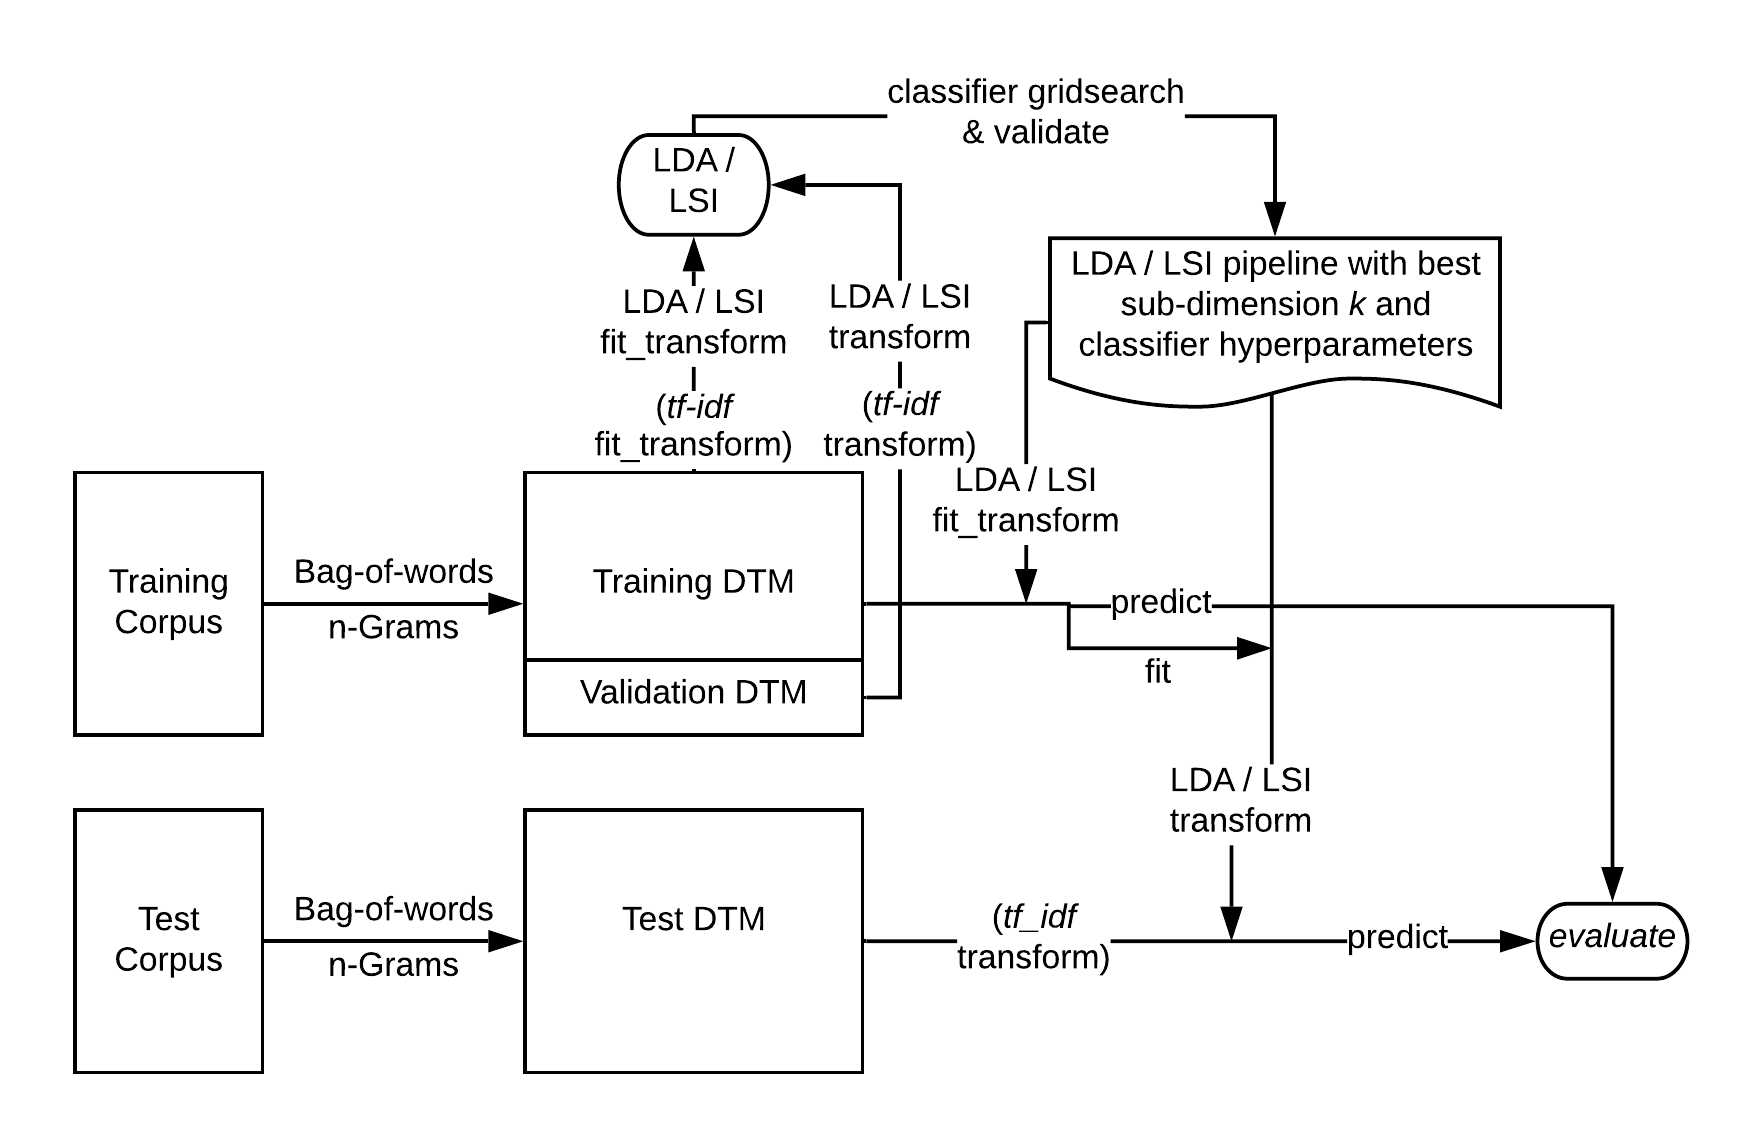
\includegraphics[width=\linewidth]{LDA_clf_workflow.png}}
  \caption{Text Classification Pipeline using LDA or LSI as a Preprocessing Step}
  \label{fig:workflow}
\end{figure}

We use a dataset of 50,000 movie reviews from the IMDb (Internet Movie Datbase) website collected by Andrew Maas (Maas et al., 2011). Each review in the dataset is labeled "positive" or "negative" according to its rating of the movie from 1 to 10. Reviews with a score of 6 or higher are labeled as positive. Half of the dataset is used as training set and the other half as test set. Both are perfectly \emph{balanced}. Our goal is to build a text classification pipeline that distinguish positive reviews from negative ones. The classifier should generalize well enough on unseen movie reviews and tag them with correct sentiment labels.

We use \emph{Logistic Regression} as our classifier. It is easy to interpret, fast to train, and perform well on large and high-dimensional datasets. The evaluation metrics we use is \emph{AUC}, as the \emph{false positive rate} against the \emph{true positive rate} (\emph{recall}). $K$, $\alpha$, regularization parameter $\lambda$ and other hyperparameters are determined by optimizing AUC on the validation set. We then refit the pipeline on the original training set, transform the test set, and report the training and test performance.

\begin{figure}[h!]
  \centering
  \fbox{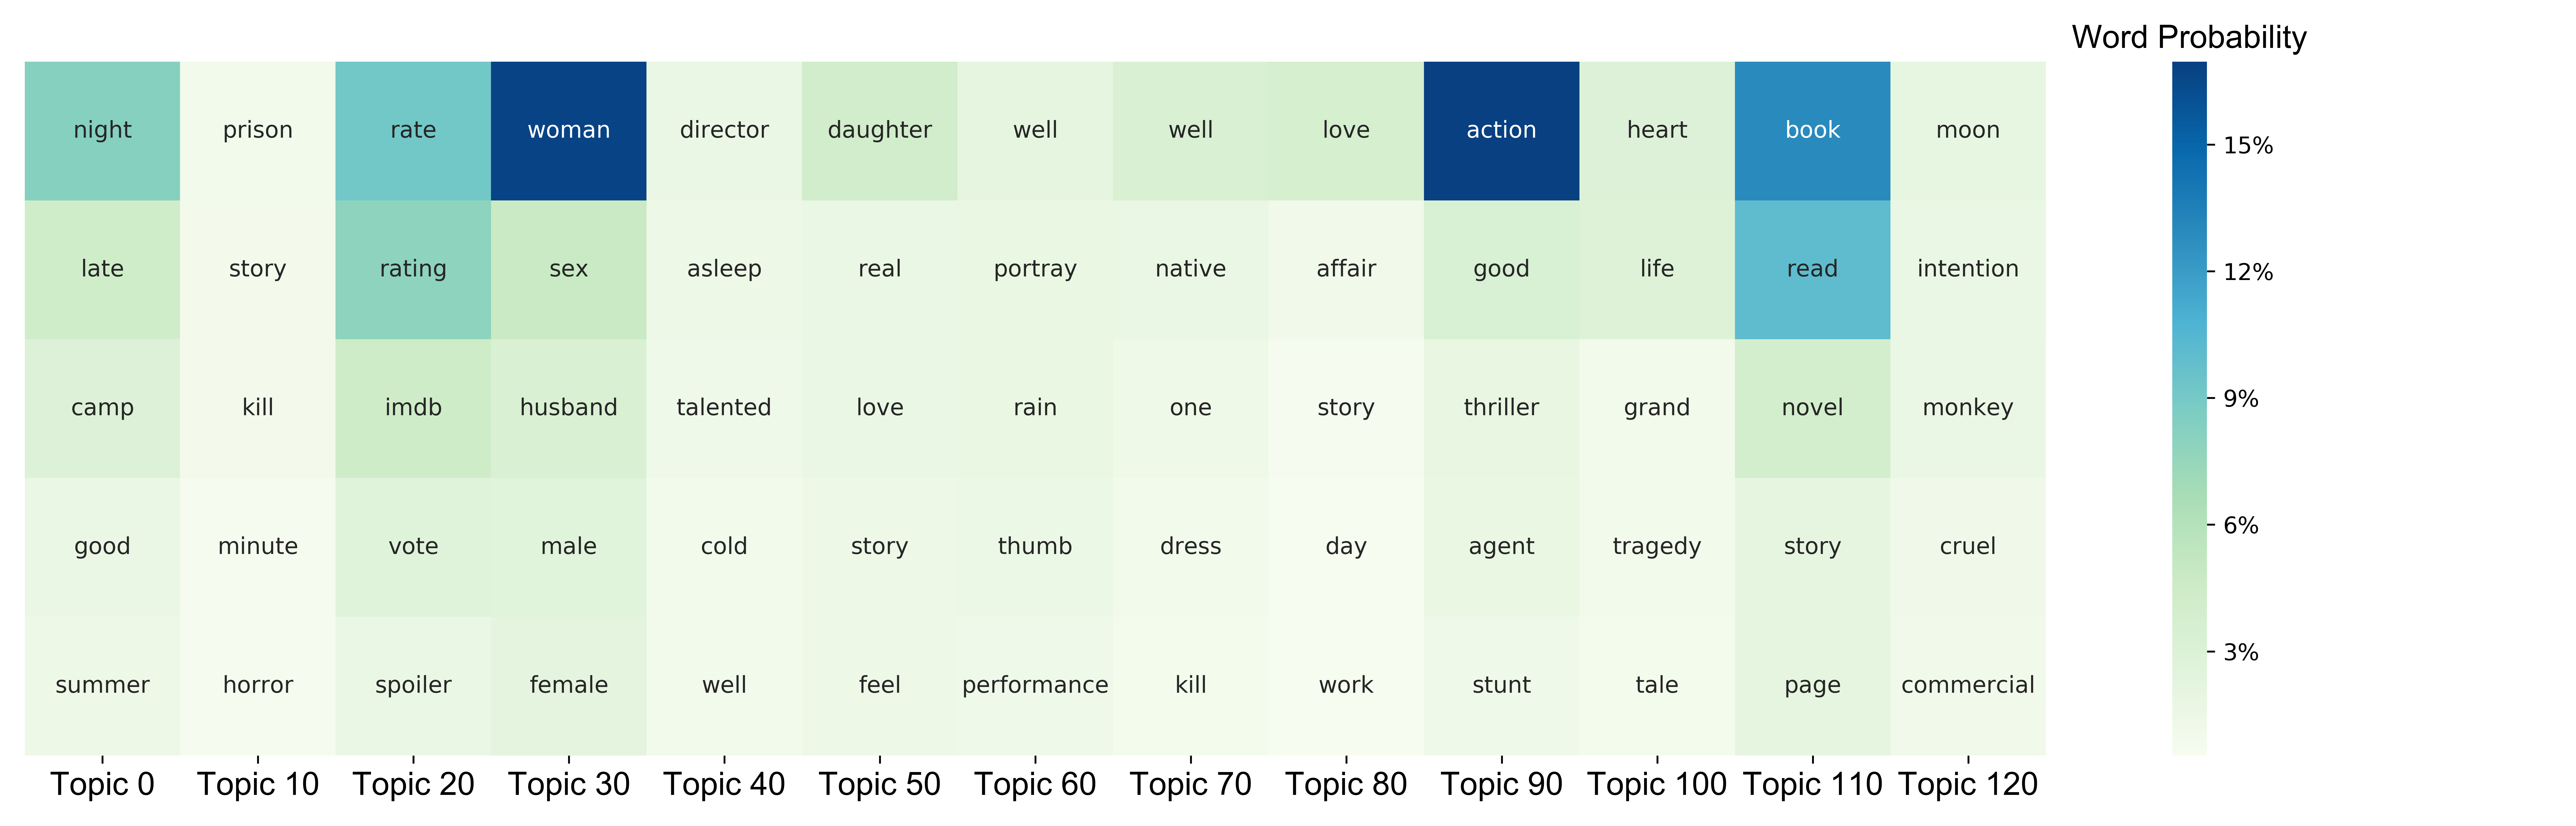
\includegraphics[width=\linewidth]{topic_word.png}}
  \caption{Illustration of the Output of a LDA model}
  \label{fig:topic_word}
\end{figure}

Figure \ref{fig:topic_word} illustrates the output of a LDA model. It shows the top 5 words (sorted by conditional probability on the corresponding topic) in each of the 13 casually chosen topics, out of the 130 topics extracted through the LDA step of the "best" classification pipeline. From these words, we imply that the latent topics are extracted based mostly on movie genres. LDA takes an unsupervised approach, and the latent semantic structure that DtM represents would not necessarily lead us to better classification results. Figure \ref{fig:pr_roc} shows the \emph{precision-recall trade-off} and the \emph{Receiver Operating Characteristic curve} of the best pipeline trained with the whole training corpus.

\begin{figure}[h!]
  \centering
  \fbox{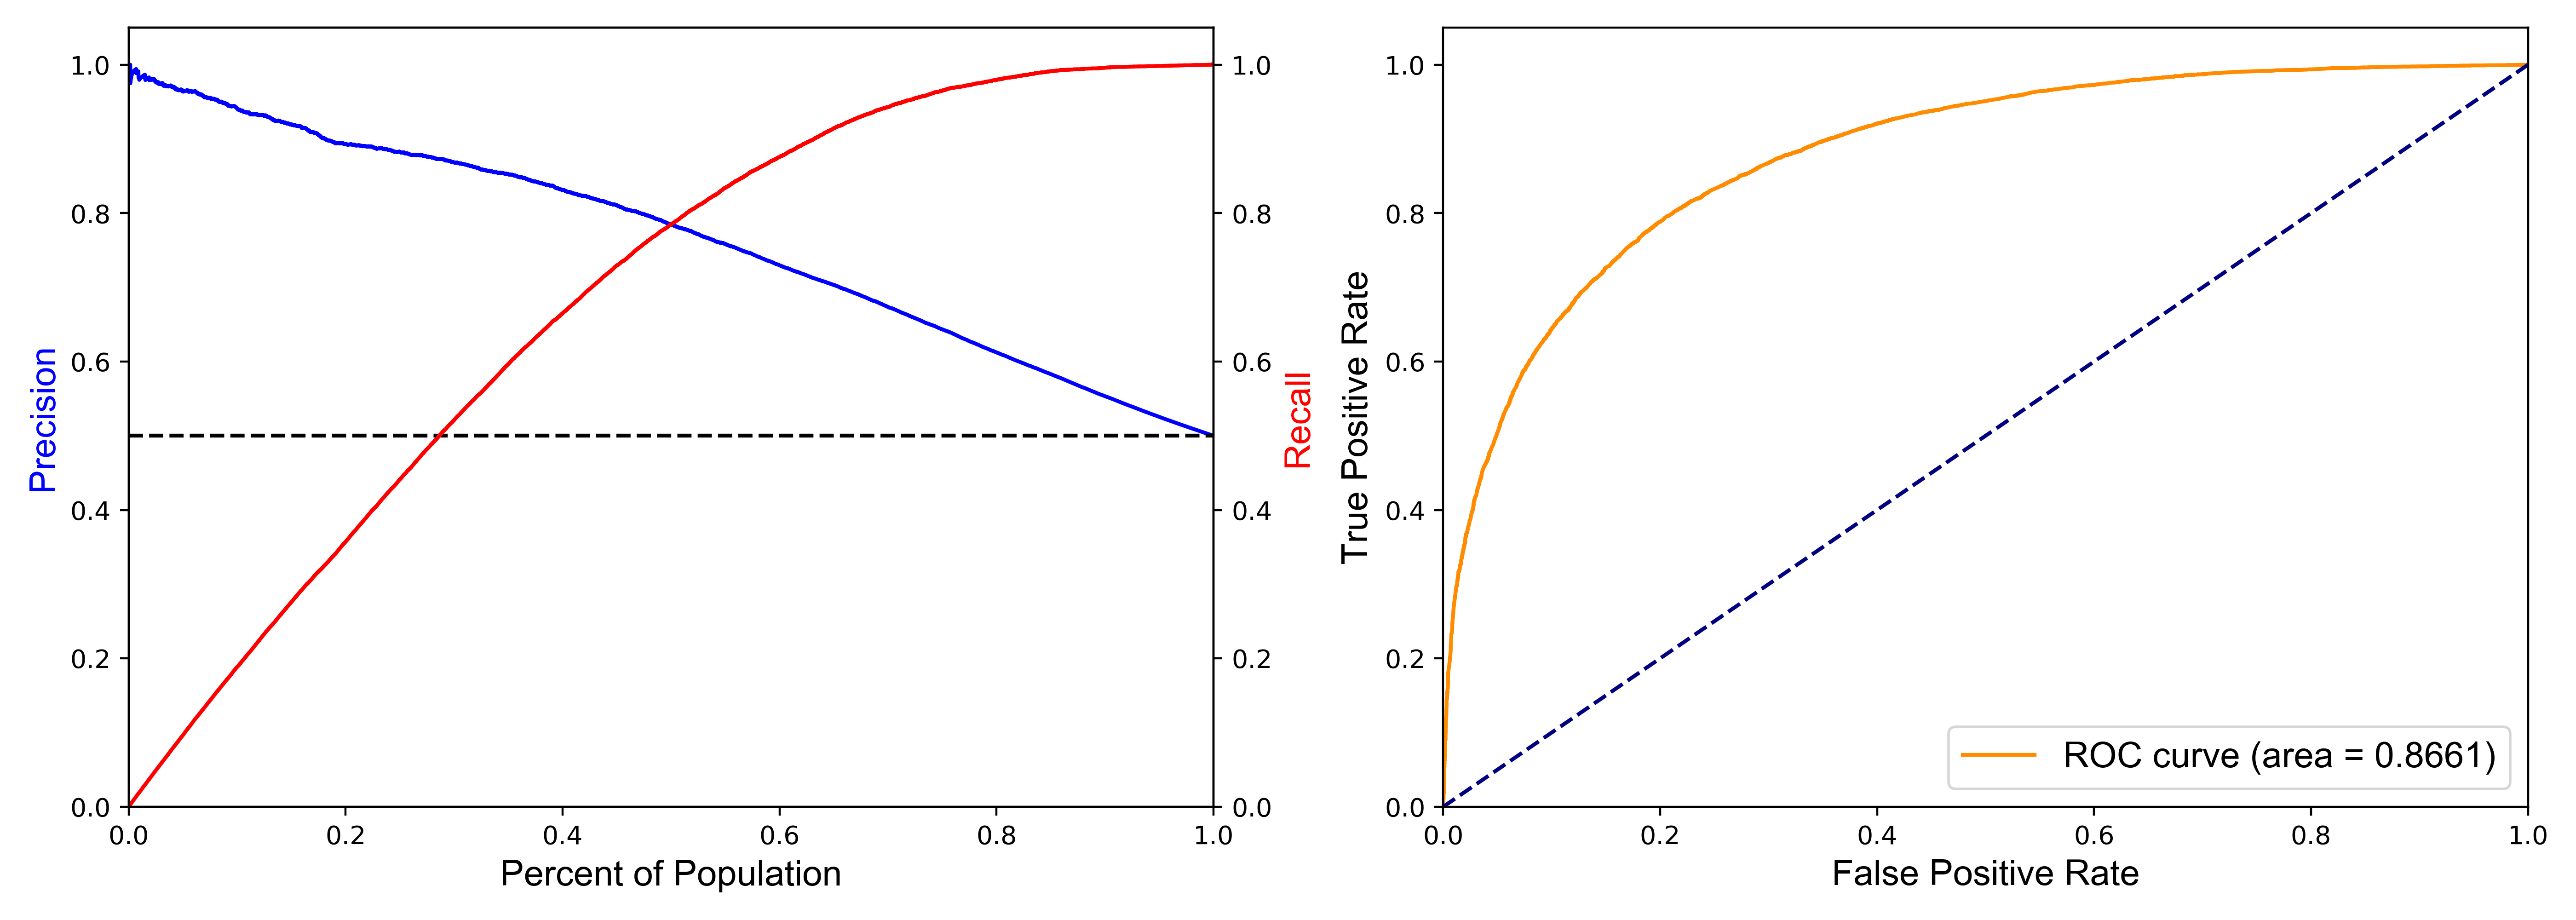
\includegraphics[width=\linewidth]{pr_roc.png}}
  \caption{Precision-recall and ROC curve for the "Best" Classifier on the whole Training Set}
  \label{fig:pr_roc}
\end{figure}

As an experiment, we also use different proportions of the original training corpus to train the classification pipeline that incorporates LDA. We also list the results from pipelines that only use \emph{tf-idf}. Figure \ref{fig:comp} compares how their test AUC, difference between test and training AUC, number of features, and training time change with increased proportions of the original training corpus used.

\begin{figure}[h!]
  \centering
  \fbox{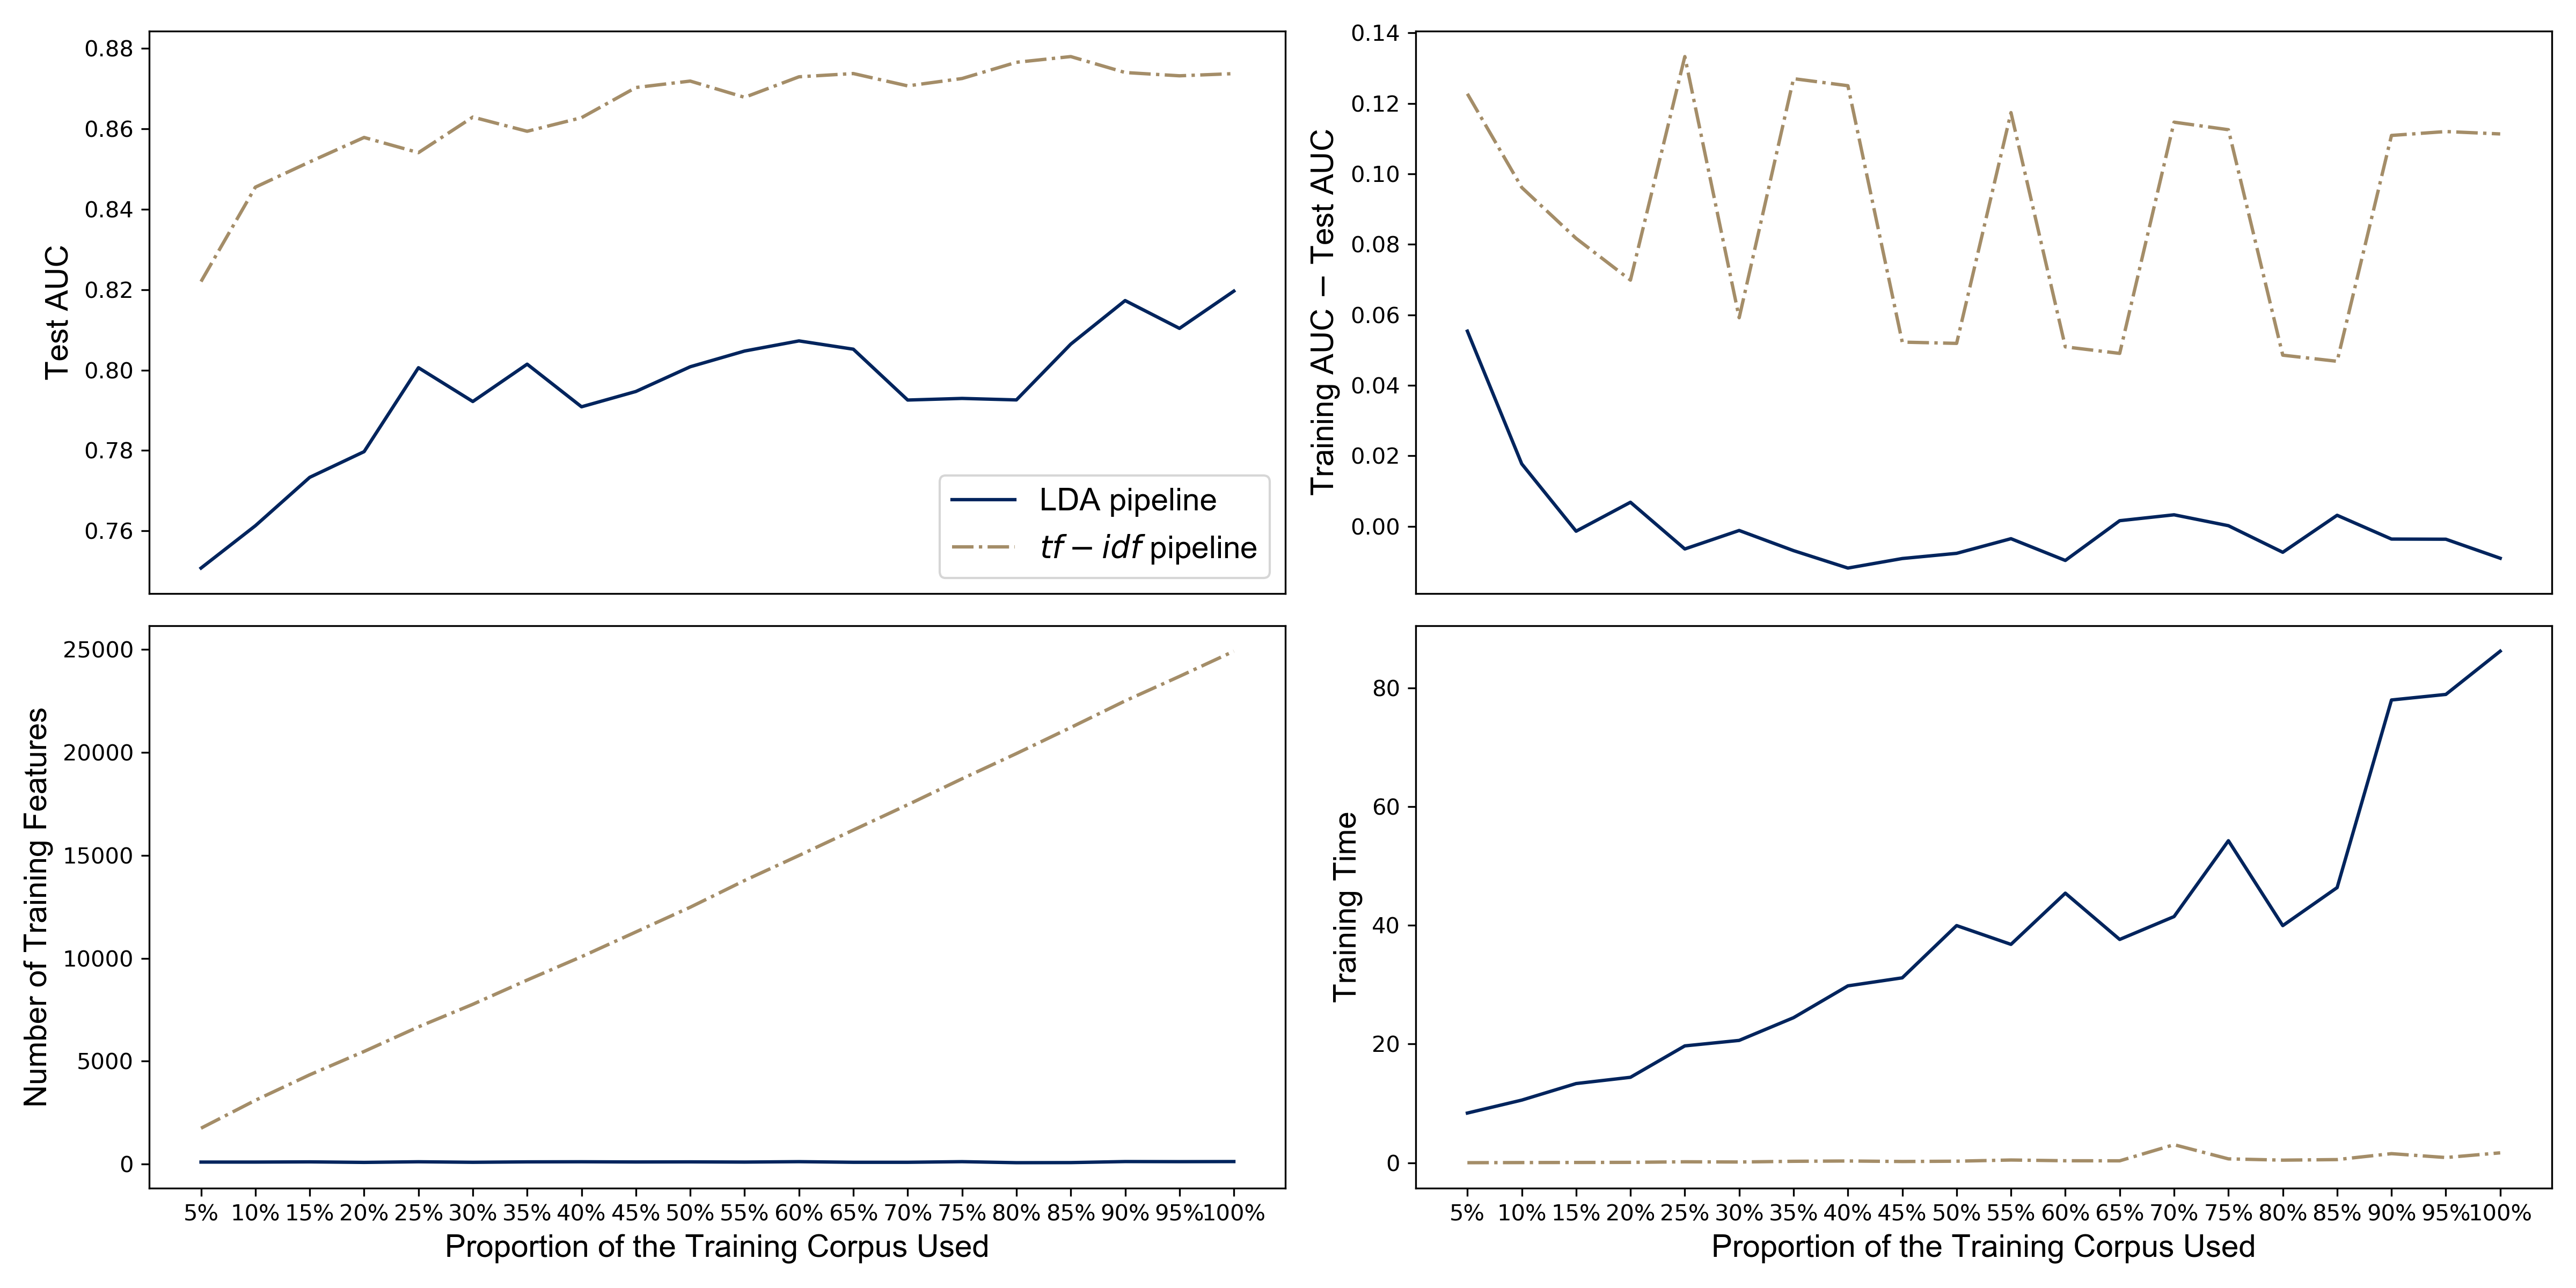
\includegraphics[width=\linewidth]{comp.png}}
  \caption{Comparing LDA Pipeline with tf-idf Pipeline on Different Training Corpus Size}
  \label{fig:comp}
\end{figure}

Apparently, test AUC for the classification pipeline with LDA preprocessing is lower by approximately 0.07. Besides, its training time is linear to the training set size, while that of the \emph{tf-idf} remains nearly constant. On the bright side, difference in test and training AUC is smaller for the LDA classification pipeline by 0.06 and is robustly decreasing with sample size. In addition, the reduction in dimensionality is very significant.


\section*{References}
\medskip

\small

[1] Blei, D. M. \ \& Ng, A. Y. \ \& Jordan, M. I. (2003) Latent Dirichlet allocation. {\it Journal of Machine Learning Research} {\bf 3}:993–1022.

[2] Dickey, J.\ (1983) Multiple hypergeometric functions: Probabilistic interpretations and statistical uses. {\it Journal of the American Statistical Association} {\bf 82}:773–781.

[3] Hofmann, T.\ (1999) Probabilistic latent semantic indexing. {\it Proceedings of the Twenty-Second Annual International SIGIR Conference}.

[4] Jordan, M.\ (1999) {\it Learning in Graphical Models}. Cambridge, MA: MIT Press.

[5] Joachims, T.\ (1999) Making large-scale SVM learning practical. In {\it Advances in Kernel Methods - Support Vector Learning}. Cambridge, MA: MIT Press.

[6] Maas, A. L. \ \&  and  Daly, R. E. \ \&  Pham, P. T. \ \&  Huang, D \ \&  Ng, A. Y. \ \& Potts, C. (2011) Learning Word Vectors for Sentiment Analysis. In {\it Proceedings of the 49th Annual Meeting of the Association for Computational Linguistics: Human Language Technologies}.

[7] Salton, G.\ \& McGill, M. (1983) In {\it Introduction to Modern Information Retrieval}. Chicago, IL: McGraw-Hill.

[8] Wei, X. \ \& Croft, W. B. (2006) LDA-based document models for ad-hoc retrieval. In {\it SIGIR}.

\end{document}